\section{Genetic and Physical mapping}

\subsection{N50 statistic}

\textbf{Contig}: A contig (from contiguous) is a set of overlapping DNA
segments.

In bottom-up sequencing projects, a contig refers to overlapping sequence
data (reads); in top-down sequencing projects, contig refers to the
overlapping clones that form a physical map of the genome that is used
to guide sequencing and assembly.

Contigs can thus refer both to overlapping DNA sequence and to overlapping
physical segments (fragments) contained in clones depending on the context. \\

\textbf{Scaffold}: it's a collection of discontinuous contigs of a given
genetic sequence.

De novo genomic assembly leads to a great number of contigs and scaffolds,
using respectively read overlaps and mate-paired analysis.

The next question is how can we put everything together.


Firstly we should have some metrics to measure the extent\footnote{Grado,
lunghezza} of the assembly.

For this purpose we use the so called \textbf{N50 statistics}.

A contig N50 is calculated by first ordering every contig by length
\textbf{from longest to shortest}.

Next, starting from the longest contig, the lengths of each contig are
summed, until this running sum equals one-half of the total length of the
genome (or, if the length of the genome is not available, you can use the sum
of the length of all contigs in the assembly).

The N50 value of a given assembly is the length of the shortest contig in this
list.

Another way to see it, is that 50\% of the genome is assembled into contigs
that are at least N50 bases long.

Generally, \textbf{high values of N50 indicate better assembly}.

The scaffold N50 is calculated in the same fashion but uses scaffolds rather
than contigs.

Like N50 you can calculate N25, N90, or any other value of N, indicating
respectively that 25\%, 90\%, or any other percentage of the genome is
assembled into contigs longer than N25, N90, etc bases.

Scaffolds and contigs with only a single read or read pair - often termed
singletons - are frequently excluded from these calculations.

Alongside with N50 very often is reported a L50 value that indicates the
number of contigs included in the list.

\paragraph*{Example} For instance, L50=350 and N50=42000 would mean that 50\%
of the genome is assembled into 350 contigs longer or equal 42000 bases. \\

\textbf{N = length of the shortest contig in the list} \\

\textbf{L = number of contigs in the list} \\

This notation $(N, L)$ is very confusing!

In fact, in some reports the two values are inverted, but common sense usually
helps. \\

\paragraph*{Gene mapping} describes the methods used to identify the locus of
a gene and the distances between genes.

The essence of all genome mapping is to place a collection of molecular
markers onto their respective positions on the genome.
Molecular markers come in all forms.
Genes can be viewed as one special type of genetic markers in the construction
of genome maps, and mapped the same way as any other markers. \\

\paragraph*{Gene Mapping VS Physical Mapping}
There are two distinctive types of "Maps" used in the field of genome mapping:
genetic maps and physical maps.

While both maps are a collection of genetic markers and gene loci,
genetic maps' distances are based on the genetic linkage information, while
physical maps use actual physical distances usually measured in number
of base pairs.

\subsection{Genetic maps}

Long before DNA sequencing, the position of genes on the genome could be
measured by considering the rate of recombination between two or more loci.

This was done even before the discovery of the function of DNA and led to the
creation of genetic maps.

Genes can be associated to particular phenotypes and can be seen from one to
the next generation.

Consider 2 loci (the positions of the genes) on the same chromosome; the
probability that they will be passed together to the next generation is
related to their reciprocal distance: the closer they are and the higher will
be the probability that they will remain together.

A \textbf{centiMorgan} is a unit of genetic distance that represents a 1\%
probability of recombination during meiosis.

E.g., if two genes are 1 cM apart, there is a 1\% chance they will break apart
during meiosis.

If two genes are 20 cM apart, there is a 20\% chance they will break apart
during meiosis.

One cM is equivalent, on average, to a physical distance of approximately 1
megabase in the human genome, but it may be different in other organisms.

The correspondence of cM and physical distance in a given organism is not
constant because genetic recombination rates vary along different parts of the
chromosomes, however it is possible to build where genes are placed on their
respective chromosomes.

Genetics maps were available before the discovery of the function of DNA.

Then, when DNA sequencing became available, many genes have been individually
sequenced and their sequences could be used as "landmarks" to assign scaffolds
to their respective chromosomes.

\subsection{Physical maps and BAC fingerprinting}
Physical maps are built on the physical DNA-base-pair distances, not
necessarily accurate to the single base, from one marker to another.

Restriction enzymes are an useful tool for making physical maps and a
restriction map is indeed a simple example of physical map.

BAC\footnote{Un Bacterial Artificial Chromosome (BAC) è un vettore artificiale
di DNA basato sul plasmide F isolato da E. coli. Il BAC si differenzia dai
normali plasmidi in quanto è in grado di trasportare regioni di DNA di
interesse molto più ampie} libraries are often used as a starting points to
make a physical maps.

Ideally, if you could do a restriction map of each BAC then you could overlap
BAC sharing similar restriction maps:

\begin{figure}[H]
  \centering
  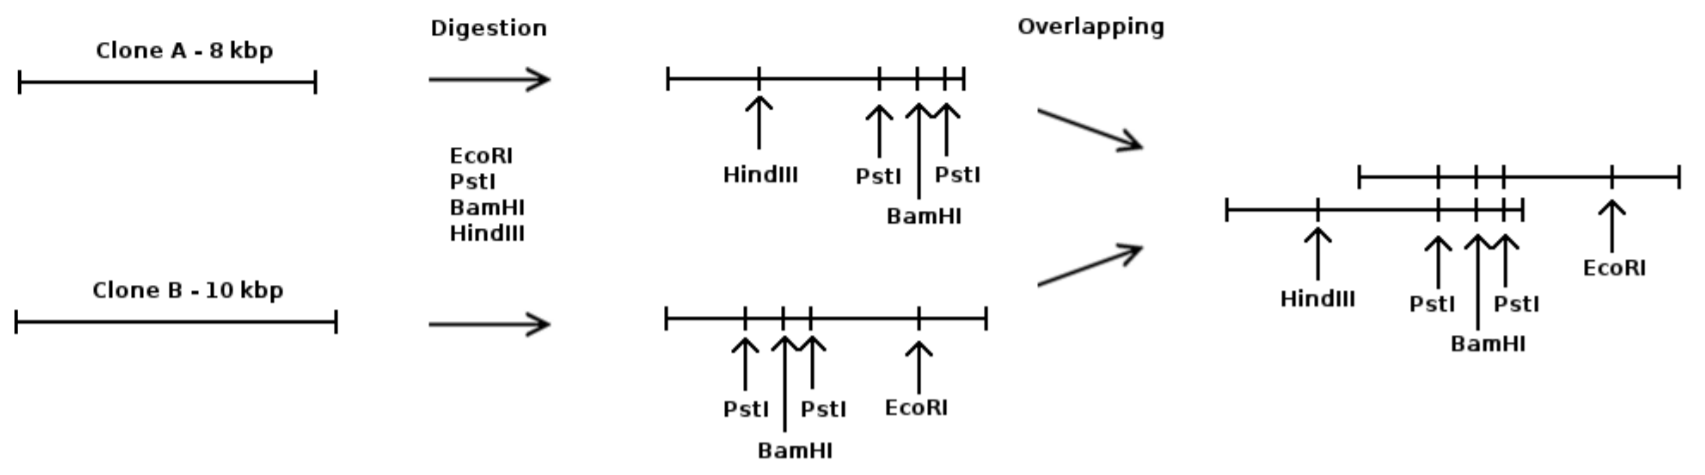
\includegraphics[scale=0.25]{physical_maps}
  \caption{}
  \label{fig:physica_maps}
\end{figure}

Recently the technology of optical mapping has become available.

If you do not have a suitable technology for optical mapping, then the
production of restriction maps is very time consuming and unsuitable for
thousands of BACs.

An alternative method called BAC Fingerprinting has been applied in many
genomic projects.

In practical terms, the DNA of each BAC is cut with restriction enzymes,
producing sets of fragments specific for the particular region of the
chromosome covered by the BAC.

Two overlapping BAC will share many fragments of the same length.

This allows to overlap BACs sharing the same fragments, even if we do not know
the relative position of each fragment.

Using fluorescent markers it is possible to use different restriction enzymes
and to label the different restriction sites with different colors, thus
increasing the specificity of the method.

\subsection{Binning: other methods for placing landmarks on a genome}

You merge a human cell with a mouse cell to pick up only cells with only one
chromosome through \textit{PCR}.

We need to map the genes in the chromosomes.
